\documentclass{beamer}
\usepackage[utf8]{inputenc}
\usepackage{xeCJK}
\usepackage{graphicx}
\usepackage{amsmath}
\usetheme{Madrid}

\setCJKmainfont{PingFang TC}

\title{輔仁大學 AI For Math}
\author{作者:盧詠涵、簡偉恆}
\date{\today}

\begin{document}

% 標題頁
\begin{frame}
  \titlepage
\end{frame}

% 預先定義所有章節,供目錄使用
\section{課程總覽}
\section{Perceptron}
\section{ADALINE 自適應線性神經元}

% 第一章:Perceptron
\section{課程總覽}
\begin{frame}{課程總覽}
\begin{enumerate}
    \item 113年學年度第二學期AI for Math系列演講
    \item 114年02月27日 潘老師 講題:感知機(The Perceptron)
    \item 114年03月06日 潘老師 講題:淺談Adaptive Linear Neuron 和Widrow-Hoff Learning
    \item 114年03月20日 潘老師 講題:The Basics of Multilayer Perceptron and Backpropagation
    \item 114年03月27日 俞讚城老師 講題:Introduction to Shannon Entropy and Cross Entropy
    \item 114年04月17日 俞讚城老師 講題:Introduction to Universal Approximation Theorems and Application in AI
    \item 114年05月08日 嚴健彰老師 講題:KAN: Kolmogorov-Arnold Networks
\end{enumerate}
\end{frame}

\section{Perceptron}
\begin{frame}{Perceptron 簡介}
  \begin{itemize}
    \item 1958 年由 Frank Rosenblatt 提出
    \item 加入可更新權重和錯誤修正學習
    \item 解決線性可分二分類問題
    \item 三層結構:輸入→隱藏→輸出
    \item 核心:誤差更正 (error-correction)
  \end{itemize}
\end{frame}

\begin{frame}{Perceptron 結構}
  \centering
  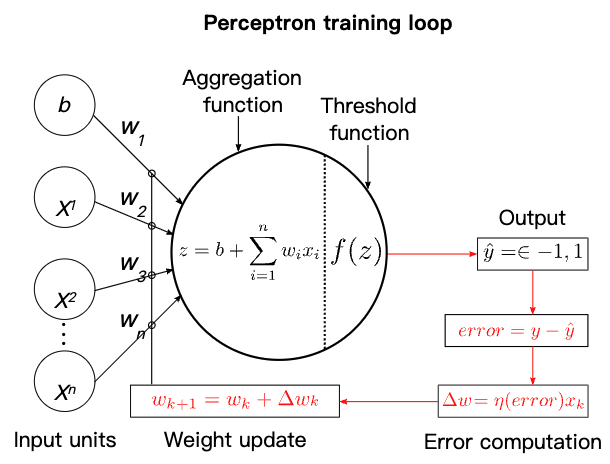
\includegraphics[width=0.8\textwidth]{perceptron_pic.png}
\end{frame}

\begin{frame}{Perceptron 的數學原理}
  \begin{itemize}
    \item 線性加權總和:$z=\sum_i w_i x_i + b$
    \item 階梯啟動函數:$\hat y=\mathrm{sign}(z)$
    \item 更新規則:$w_i\leftarrow w_i+\eta(y-\hat y)x_i$
    \item 收斂保證:線性可分時有效
  \end{itemize}
\end{frame}

\begin{frame}{Perceptron 示意圖}
  \centering
  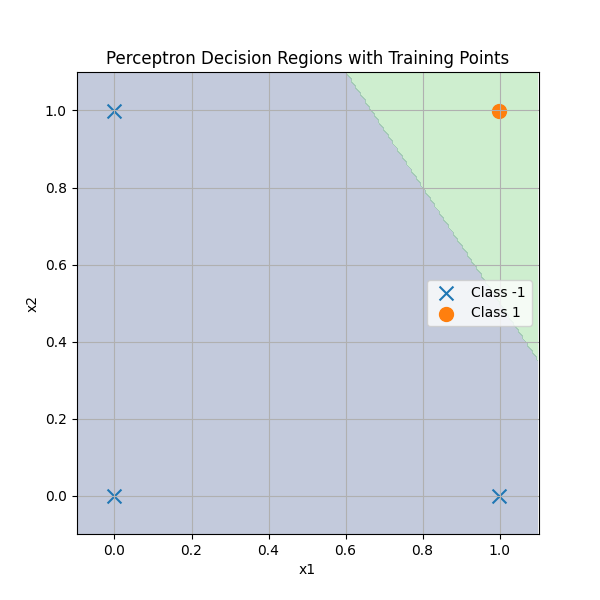
\includegraphics[width=0.7\textwidth]{Perceptron.png}
\end{frame}

% 第二章:ADALINE
\section{ADALINE 自適應線性神經元}
\begin{frame}{ADALINE 自適應線性神經元}
  \centering
  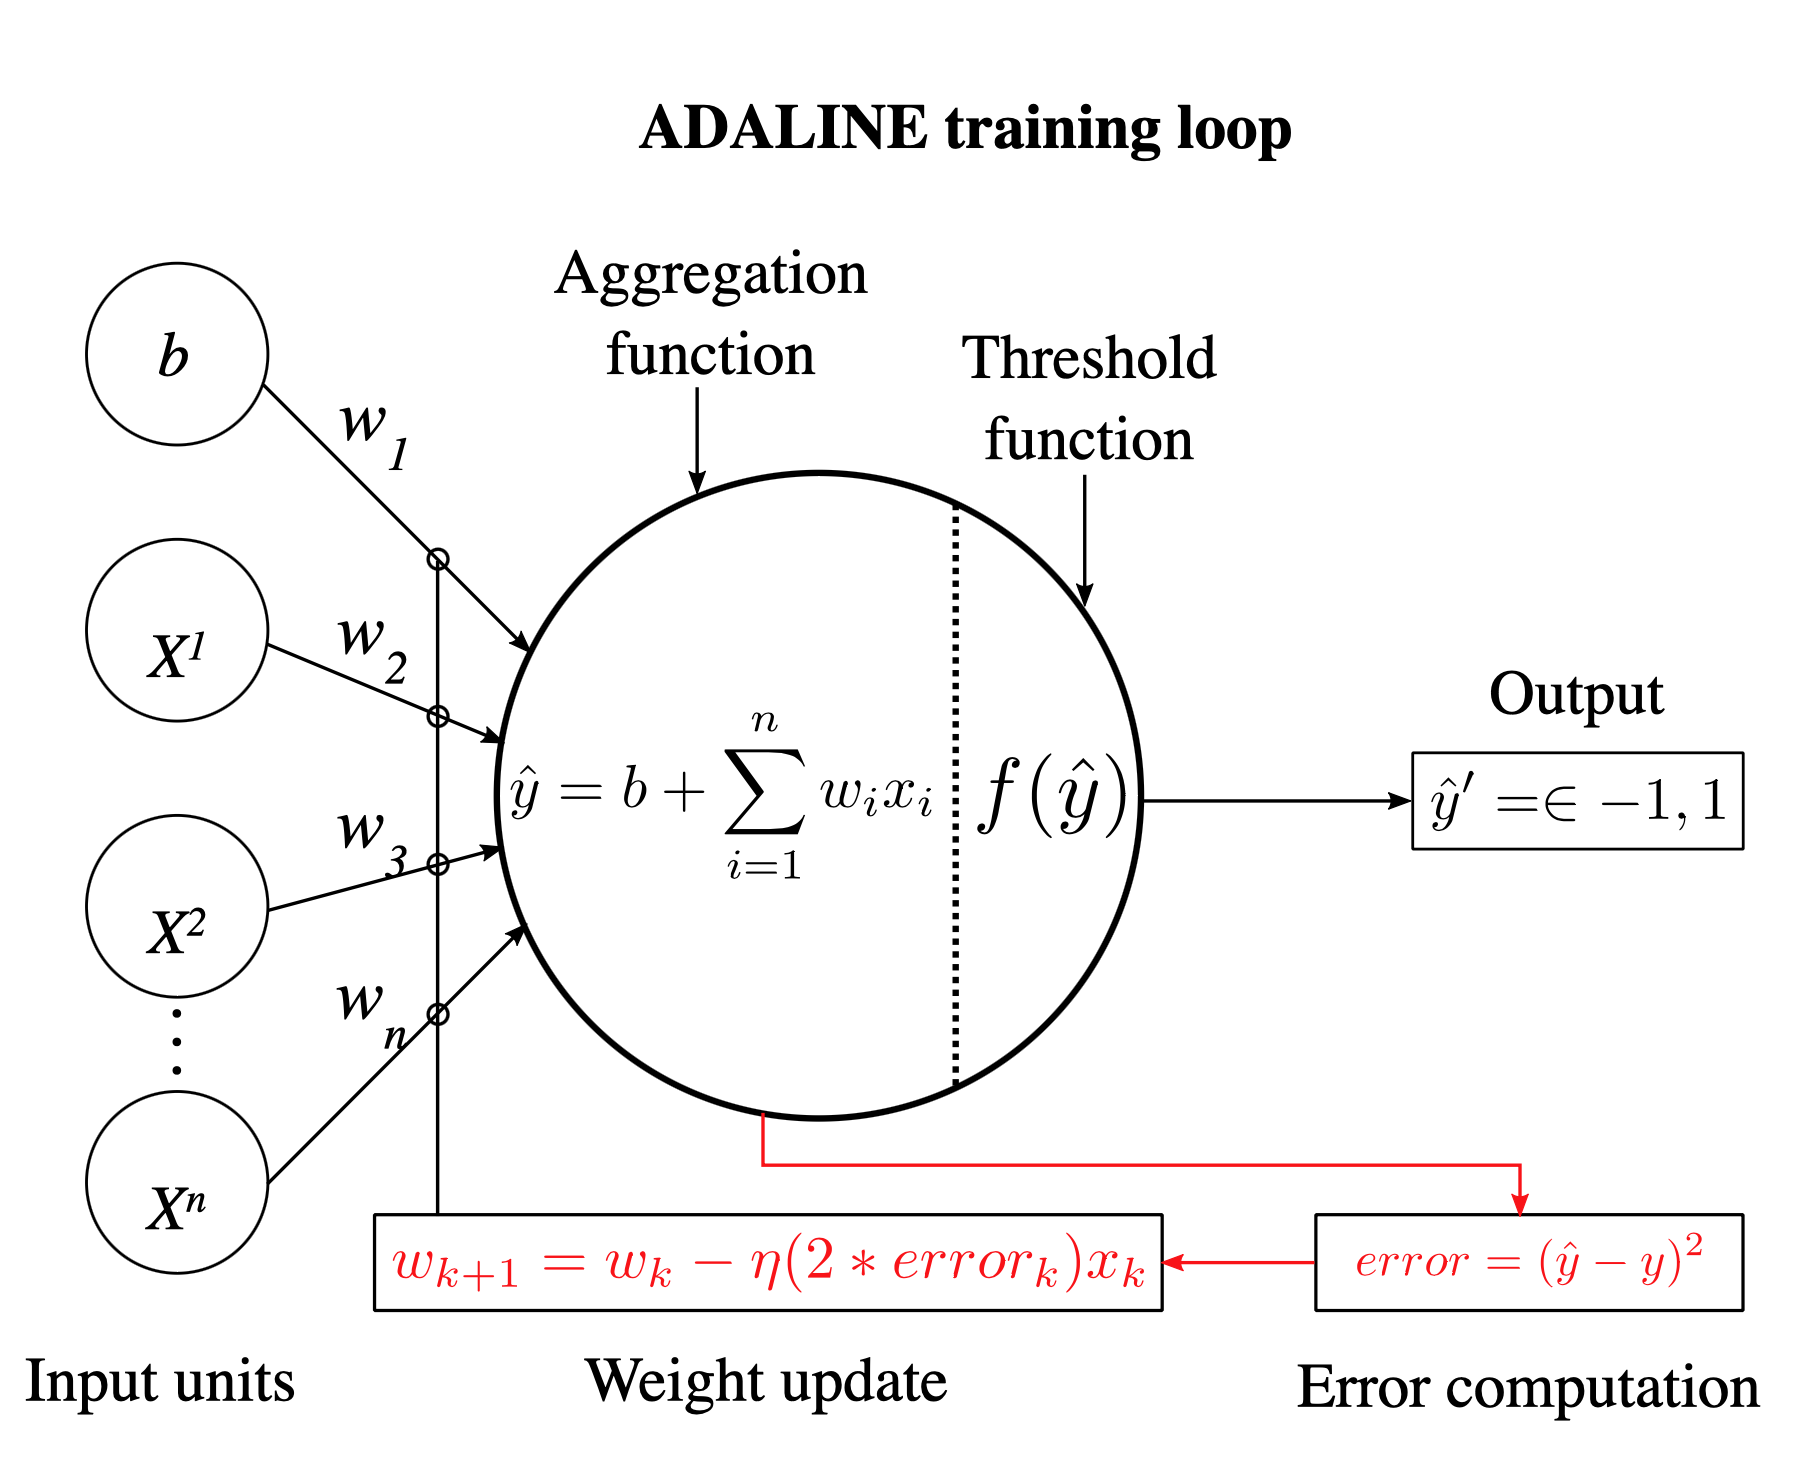
\includegraphics[width=0.7\textwidth]{ADALINE_picture.png}
\end{frame}

\begin{frame}{Overview}
  \begin{itemize}
    \item 發明者:Widrow \& Hoff (1959)
    \item 目標:最小化均方誤差 (MSE)
    \item 特點:線性輸出,連續可微
    \item 演算法:梯度下降 (Gradient Descent)
    \item 優勢:收斂穩定、更新平滑
  \end{itemize}
\end{frame}

\begin{frame}{ADALINE 數學形式}
  \[
    \hat y=\mathbf{w}^\top\mathbf{x}+b
  \]
  \[
    \mathrm{MSE}=\frac1n\sum_i(y_i-\hat y_i)^2
  \]
  \[
    w\leftarrow w-\eta(y-\hat y)x
  \]
\end{frame}

\begin{frame}{訓練演算法}
  \begin{itemize}
    \item 計算加權和:$\hat y$
    \item 計算誤差:$(y-\hat y)^2$
    \item 權重更新:$w\leftarrow w-\eta(y-\hat y)x$
  \end{itemize}
\end{frame}

\begin{frame}{應用場景}
  \begin{itemize}
    \item 自適應濾波 (Adaptive Filtering)
    \item 噪音消除 (Noise Cancellation)
    \item 時序預測 (Time Series Prediction)
    \item 自動控制系統 (Control Systems)
  \end{itemize}
\end{frame}

\end{document}
